\documentclass[UTF8]{ctexart}

\usepackage{WeeklyReport}
\usepackage{graphicx}
\usepackage{amsmath}
\usepackage{amssymb}

\title{周报10}
\author{傅阳烨}
\date{\today}

\begin{document}
\maketitle
% \tableofcontents
\section{学习内容}
\begin{itemize}
    \item DomainNet 数据集测试(待续……)
    \item 阅读 Partial Domain Adaptation 相关文章
\end{itemize}

\section{学习收获}
\subsection{DomainNet 数据集测试情况}
这部分的代码已经写好了,主要做的调整在于读取图片时的缩放大小和 batch size,不过服务器目前有人在用,所以实验暂时推迟一下。
尽管如此,在读取数据的时候出现了 MemoryError,代码逻辑本身没有问题,但由于增大了读取数据的放缩大小并且数据集本身很大,在转换为 float 类型时会出现内存不足的情况,
说明不能一次性将整个数据集读取进内存,而分批读取数据可能会影响随机取样,这个问题正在想办法解决。

然而当前最主要的还是多测试一些想法,更大数据集上的测试应该放在后面一些。

\subsection{Learning to Transfer Examples for Partial Domain Adaptation (CVPR2019)}

找到了一篇与部分领域自适应相关的文章,主要是想应用到特征选取上,不过这篇文章所提到的 partial 实际上是指 label space 而不是 feature space。

文章所研究的问题属于 target 类别与 source 类别不相同的情况,target 的 label space 未知,
而假定 target domain 的 label space 是 source domain 的超集。

作者提出了 Example Transfer Network (ETN) 用于借助可迁移性(transferability)学习与 target 相关的 example(或者说类别属于 target 的 label space 的 example)。

\subsubsection{Motivation}
如图 \ref{fig:Negative},文章想要解决的是主流方法中存在的负迁移的问题,
传统方法由于 source 中与 target 不符的 class 的影响(target 的 label 是未知的,所以 target 具有哪些 class 也是未知的),
并且 shared class 和 outlier class 中均会出现不相关的 example,容易造成负迁移,迁移过的模型表现可能还不如迁移前的模型,
所以作者提出的 ETN 目的在于处理 shared class 和 outlier class 中与 target 相关的 example。

\begin{figure}[ht]
    \centering
    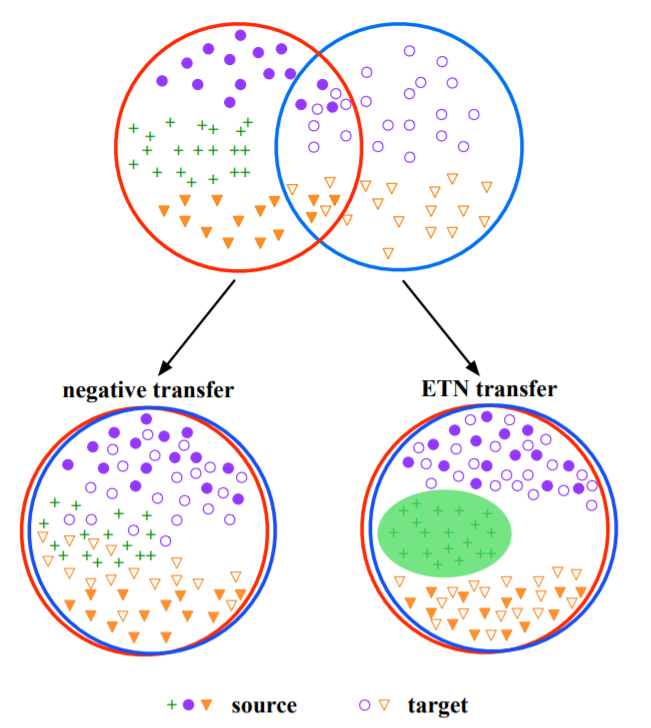
\includegraphics[scale=0.3]{Week10_Negative.png}
    \caption{PDA 与 ETN}
    \label{fig:Negative}
\end{figure}

\subsubsection{思路}
与普通的领域适应问题相同,假设存在一个源域 $\mathcal{D}_s$ 和一个目标域 $\mathcal{D}_t$,
且源域的类标签所在空间 $\mathcal{C}_s$ 与目标域的类标签所在空间 $\mathcal{C}_t$ 满足 $\mathcal{C}_s \supset \mathcal{C}_t$。

使用一个可迁移特征提取器 $G_f$ 和自适应分类器 $G_y$ 用于缩减域之间的分布差异。
训练的过程当作一个 two-player 的 minimax game(感觉相当于是对抗训练),两个 player 分别
为 $G_d$ 和 $G_f$,其中 $G_d$ 要根据 feature 区分样本来自 source 还是 target(常见的方法),
$G_f$ 则要欺骗 $G_d$(常见的对抗训练思想)。

在极大极小值优化的过程中,域无关的特征会被提取出来,所使用的 loss 是对抗训练时常用的 loss:

$$
E(\theta_f, \theta_y, \theta_d) = \frac{1}{n_s}\sum_{x_i\in\mathcal{D}_s}L_y(G_y(G_f(x_i)), y_i) - \frac{1}{n_a}\sum_{x_i\in\mathcal{D}_a}L_d(G_d(G_f(x_i)), d_i)
$$

其中 $\mathcal{D}_a = \mathcal{D}_s \cup \mathcal{D}_t$ 是源域和目标域的并集,
$L_y$ 和 $L_d$ 是 cross entropy loss。

上面都是一些已有的网络结构,而 outlier class 的存在会使得迁移效果下降,
于是作者的创新点在于提出了一个可迁移加权框架(transferability weighting framework),
用 $w(x_i^s)$ 表示 source 中每个 example $x_i^s$ 的权重,在计算 loss 的时候,
将这些 example 的权重也放进去(包括 $G_d$ 和 $G_y$ 的 loss)。按作者的说法,这样可以区分出 irrelevant 的 source example。

为了解决 shared class 不确定的问题,作者利用生成样本的 entropy loss 去对 target example 的标签预测不确定性进行量化:

$$
\hat{y}_j^t = G_y(G_f(x_j^t)) \in \mathbb{R}^{|\mathcal{C}_s|}
$$

$$
H(G_y(G_f(x_j^t))) = -\sum_{c=1}^{|\mathcal{C}_s|} y_{j, c}^t \log y_{j, c}^t
$$

由此得到如下的 loss function:

$$
E_{G_y} = \frac{1}{n_s}\sum_{i=1}^{n_s} w(x_i^s)L(G_y(G_f(x_i^s)), y_i^s) + \frac{\gamma}{n_t}\sum_{j=1}^{n_t} H(G_y(G_f(x_j^t)))
$$

$$
E_{G_d} = - \frac{1}{n_s}\sum_{i=1}^{n_s} w(x_i^s)\log(G_d(G_f(x_i^s))) - \frac{1}{n_t}\sum_{j=1}^{n_t}\log(1 - G_d(G_f(x_j^t)))
$$

其中 $\gamma$ 是超参数,用于在带标签的 source example 和不带标签的 target example 之间折衷。

可迁移加权框架的训练过程相当于是驻点 $(\hat{\theta}_f, \hat{\theta}_y, \hat{\theta}_d)$ 的求解过程:

$$
(\hat{\theta}_f, \hat{\theta}_y) = {\arg \min}_{\theta_f, \theta_y} E_{G_y} - E_{G_d}
$$

$$
(\hat{\theta}_d) = \text{arg min}_{\theta_d} E_{G_d}
$$

现在还需要求解加权向量 $w$,作者提出了一个辅助的域判别器 $\tilde{G}_d$,同样是被训练用于区分 source domain 和 target domain,
使用相似的 loss,但是不参与对抗训练,即 $G_f$ 的训练不用于 confuse $\tilde{G}_d$。
作者指出这样的 $\tilde{G}_d$ 可以对 source example 的可迁移性进行量化。

文章还提出了一个辅助的 label predictor $\tilde{G}_y$,用于得到可分离的权重(?)。

最终得到权重如下:

$$
w(x_i^s) = 1 - \tilde{G}_d(G_f(x_i^s))
$$

为了保证权重之和为1,对权重进行 normalize:

$$
w(x) = \frac{w(x)}{\frac{1}{B}\sum_{i=1}^B w(x_i)}
$$

其中 $B$ 表示 batch size。

\begin{figure}[ht]
    \centering
    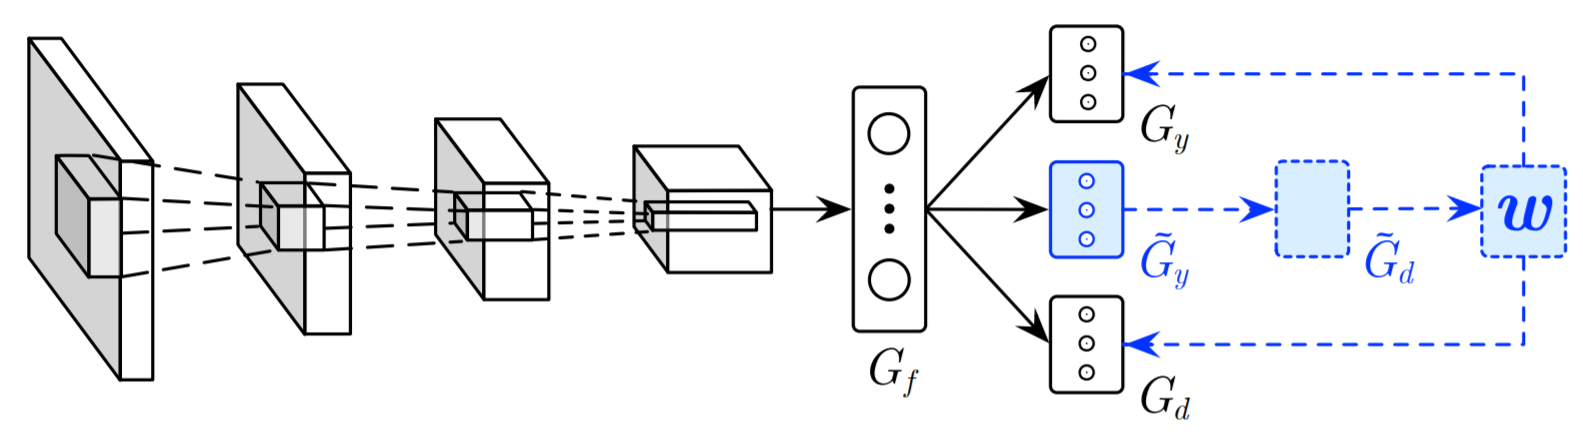
\includegraphics[scale=0.3]{Week10_ETN.png}
    \caption{ETN 结构}
    \label{fig:ETN}
\end{figure}

最后 ETN 的整体网络结构如图 \ref{fig:ETN} 所示,其中 $G_f$ 是特征提取器,$G_y$ 是源域分类器,
$G_d$ 是用于 domain alignment 的域判别器(参与了对抗训练),$\tilde{G}_d$ 是辅助的域判别器(不参与对抗训练),
用于量化每个 source example 的 $w$。$\tilde{G}_y$ 表示辅助的类标签预测器,用于将 discriminative 的信息 encode 后传给 $\tilde{G}_d$。
图中的蓝色部分是作者提出的新结构。

\subsubsection{实验}
作者在 Office-31、Office-Home 和 ImageNet-Caltech 三个数据集上进行了测试,所得到的结果如图 \ref{fig:test} 所示。

\begin{figure}[ht]
    \centering
    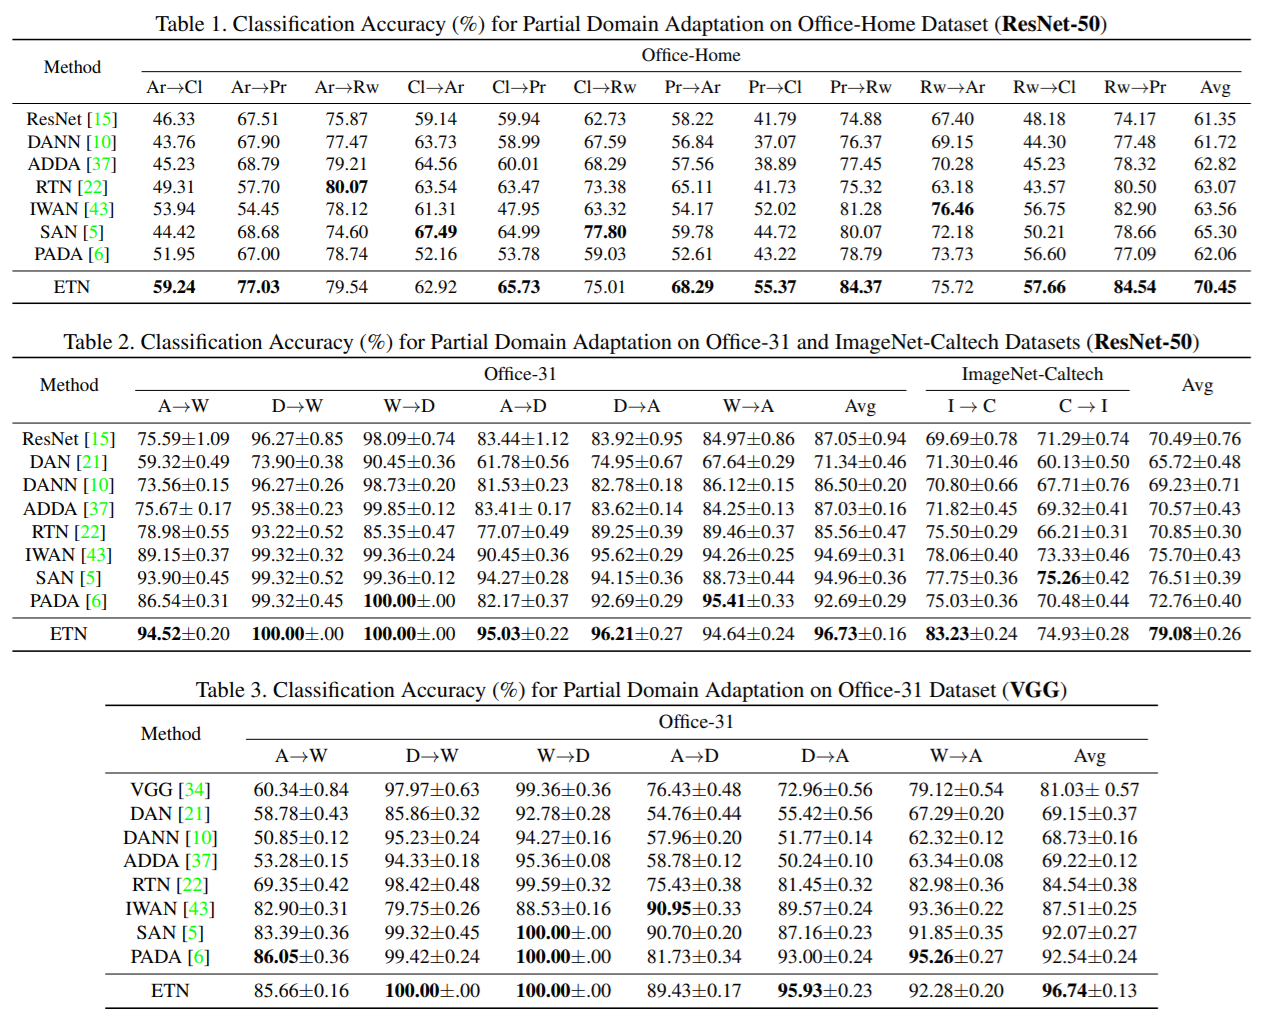
\includegraphics[scale=0.38]{Week10_test.png}
    \caption{ETN 实验结果}
    \label{fig:test}
\end{figure}

从结果上可以看到,ETN 在部分域之间的迁移效果比原先的模型更好。

\subsubsection{小结}
尽管文章是从 label space 的角度去分析 partial domain adaptation 的,
但其中使用的 weighting function 可以放在特征选择中使用,可迁移性的问题也可以放在特征层面去讨论,
甚至在多源领域适应中,可以分别分析各个 source 与 target 之间的可迁移性,对 source 进行提炼。

\section{启发}
\begin{enumerate}
    \item 提取 example 的过程可以运用到多源领域自适应的任务中,将特征与 target 相似或匹配的 source domain 中的 example 提取出来进行训练
    \item 文章所提出的可迁移性的概念,可以放到特征上去考虑,而文章给出的可迁移量化方法,可以用于评价源域与目标域特征的相关性
    \item 尽管文章是从标签有偏差的角度去考虑的,但如果这篇文章的类别看作多源领域自适应中的特征,则可以用同样的方法提取 example,或者生成特征选择的权重
\end{enumerate}
\section{疑问/困难}
\begin{enumerate}
    \item 按照 Digit-Five 的套路去编写的 DomainNet 数据集测试代码,运行时内存占用过大,出现 MemoryError,读取数据的方式需要改进
    \item 一张张去读取 DomainNet 数据集比较慢,完整读取一次大约需要一小时,尝试过转化为 json 再读取,但效果并不理想(所需时间几乎相同)
    \item Partial Domain Adaptation 的文章使用了对抗训练的方法,而对抗训练是比较困难的
\end{enumerate}
\end{document}
